\documentclass[a4paper, 12pt]{article}

%\usepackage{cmap}
\usepackage[T2A]{fontenc}
\usepackage[utf8]{inputenc}
\usepackage[english, russian]{babel}
\usepackage{graphicx}
\usepackage[top=1in, bottom=1in, left=3.2cm, right=2.6cm]{geometry}
\graphicspath{./}
\usepackage{biblatex}
\addbibresource{lib.bib}
\linespread{1.5}
\usepackage{ragged2e}
\justifying
\usepackage{listings}
\usepackage{color}


\begin{document}
	
\begin{titlepage}
	\fontsize{12pt}{12pt}\selectfont
	\begin{figure}[t!]
		\centering
		
\includegraphics[scale=0.8]{bmstu}
	\end{figure}
	
	\noindent\rule{15cm}{3pt}
	\newline\newline
	\noindent 
	ФАКУЛЬТЕТ 
	\underline{«Информатика и системы управления»} \newline\newline
	
	\noindent КАФЕДРА \underline{«Программное обеспечение ЭВМ и информационные технологии»}\newline\newline\newline\newline\newline
	
	\centering {\Large Отчет по лабораторной работе № 11-13}
	\vspace{4mm}
	
	\centering {\Large По курсу: "Функциональное и логическое программирование"
		\vspace{8mm}	
		
		}
	\vspace{8mm}
	
	
	\begin{flushright}
		{\small	Студент:\\ Турсунов Жасурбек Рустамович \\ Группа: ИУ7-66Б
			\vspace{3mm}
			\\Преподователи: \\ Толпинская Наталья Борисовна \\ Строганов Юрий Владимирович}
	\end{flushright}
	
	\begin{center}
		\vfill
		Москва, \the\year
		~г.
	\end{center}
\end{titlepage}

\tableofcontents
\clearpage
\newpage

\textbf{Цель работы:} Познакомится со средой Visual Prolog, познакомится со структурой программы: способом запуска и формой вывода результатов.
\\ \hspace*{5mm} \textbf{Задачи работы:} изучить принципы работы в среде  VisualProlog, возможность получения однократного и многократного результата, изучить базовые конструкции языка Prolog, структуру программы программы Prolog, форму ввода исходных данных и вывода результатов работы программы. 

\section*{Введение}
\addcontentsline{toc}{section}{Введение}

\hspace*{5mm} Программа на Prolog представляет собой базу знаний и вопрос. База знаний содержит истинные значения, используя которые программа выдает ответ на вопрос. В процессе поиска ответа программа рассматривает все возможные альтернативные решения и находит все возможные значения переменных, при которых на поставленный вопрос можно ответить “ДА”.
\\ \hspace*{5mm} Основным элементом языка является терм: константа, переменная или составной терм. Составной терм является предикатом. Программа представляет набор фактов и правил. 
\\ \hspace*{5mm}Факты представляют собой составные термы, с помощью которых фиксируется наличие истинности между объектами предметной области – аргументами терма.
\\ \hspace*{5mm} Правила являются обобщённый формулировкой условий истинности отношения между объектами предметной области (аргументами терма), которое записано в заголовке правила. Условие истинности этого отношения является телом правила. Заголовок правила отделяется от тела правила символом «:-», правило завершается символом «.». Заголовок правила – это предикат. Тело правила может быть представлено последовательностью предикатов.

Основной элемент языка-терм.
\\ Терминология:
\begin{enumerate}
	\item Простой
	\begin{itemize}
		\item Константа(с маленькой буквы);
		\begin{itemize}
			\item Символ;
			\item Число.
		\end{itemize}
		\item Переменная (с большой буквы);
		\begin{itemize}
			\item Именованная;
			\item Анонимная.
		\end{itemize}
		\item Составной (пример $f(t_1, t_2,..., t_n)$). Где F-функтор (имя отношения между объектами)
	\end{itemize}
\end{enumerate}

\textbf{Особенность использования переменных}
\\ \hspace*{5mm} Именованные переменные уникальны в предикатах одного предложения, анонимные уникальны везде. Анонимные переменные не возвращают значение. Переменной можно обозначить любой объект. При описании переменная может потерять свое значение, но потом его можно вернуть.
\textbf{Структура программы}
Программа состоит из разделов:
\begin{enumerate}
	\item Domains - отношение имен и структур объектов (не обязателен);
	\item Predicates – описание предикатов (названий отношений между объектами);
	\item Clauses – база знаний;
	\item Goal – Раздел целевых утверждений.
\end{enumerate}
Программа состоит из предложений:
\begin{enumerate}
	\item Факт (безусловная истина, формулируется составным термом)- частный случай правил;
	\item Правила (условная истина, способ порождения новых фактов на основе имеющихся).
\end{enumerate}

Вопрос:
\begin{enumerate}
	\item Конъюнктивный (B1, B2, B3);
	\item Дизъюнктивный (B1; B2; B3).
\end{enumerate}

\clearpage
\newpage


\definecolor{codegreen}{rgb}{0,0.6,0}
\definecolor{codegray}{rgb}{0.5,0.5,0.5}
\definecolor{codepurple}{rgb}{0.58,0,0.82}
\definecolor{backcolour}{rgb}{0.95,0.95,0.92}

\lstdefinestyle{mystyle}{
	backgroundcolor=\color{backcolour},   
	commentstyle=\color{codegreen},
	keywordstyle=\color{magenta},
	numberstyle=\tiny\color{codegray},
	stringstyle=\color{codepurple},
	basicstyle=\ttfamily\footnotesize,
	breakatwhitespace=false,         
	breaklines=false,                 
	captionpos=b,                    
	keepspaces=true,                 
	numbers=left,                    
	numbersep=5pt,                  
	showspaces=false,                
	showstringspaces=false,
	showtabs=false,                  
	tabsize=4
}

\lstset{style=mystyle}

\section*{Задание 1}
\addcontentsline{toc}{section}{Задание 1}
Разработать свою программу - "Телефонный справочник". Протестировать работу программы.
\begin{lstlisting}
domains
	NAME=symbol
	NUM=string
	AREA=integer
	CITY=string
	STREET=string
	HOUSE=integer

predicates
	likes(symbol,symbol)
	abonent(NAME,NUM)
	abonname(NAME,NUM)
	abonnum(NAME,NUM)
	house(NAME,AREA,CITY,STREET,HOUSE)
	housesAddr(NAME,CITY,STREET,HOUSE)
	housesAREA(NAME,AREA)
	mult(NAME,NUM,CITY)

clauses
	likes(ellen,tennis).
	likes(john,football).
	likes(tom,baseball).
	likes(eric,swimming).
	likes(mark,tennis).
	likes(bill,Activity):-likes (tom, Activity).

	abonent(alex,"1111111").
	abonent(alex,"1112121").
	abonent(ivan,"2222222").
	abonent(petr,"3333333").
	abonent(semen,"444444").
	abonent(evgen,"555555").
	abonent(dima,"6666666").
	abonent(semen,"777777").
	abonent(oleg,"888888").
	abonent(roman,"9999999").

	house(alex,2500,"Moscow","Baker",140).
	house(alex,560,"London","Baker",221).
	house(alex,70,"NY","Baker",14).
	house(ivan,2500,"Moscow","Lyubanka",10).
	house(semen,56,"London","Tsentranly",14).
	house(dima,700,"NY","Tsemntr",221).


	abonname(NAME,NUM):-abonent(NAME,NUM).
	abonnum(NAME,NUM):-abonent(NAME,NUM).
	housesAddr(NAME,CITY,STREET,HOUSE):-house(NAME,_,CITY,STREET,HOUSE).	
	housesAREA(NAME,AREA):-house(NAME,AREA,_,_,_).
	mult(NAME,NUM,CITY):-house(NAME,_,CITY,_,_),abonent(NAME,NUM).



goal
	abonname(alex,NUM).
	%housesAddr(alex,CITY,STREET,HOUSE).
	%housesAREA(alex,AREA).	
	%mult(alex,NUM,ADDRESS).
	%house(alex,_,ADDRESS),abonent(alex,NUM).
	
\end{lstlisting}
Результат работы программы\\\\
\hspace*{-10mm}\begin{tabular}{ | l | l | }
	\hline
	\textbf{Вопрос} & \textbf{Результат} \\ \hline
	abonname(alex,NUM). & NUM=1111111/ NUM=1112121/ 2 Solutions\\ \hline
	housesAddr(alex,CITY, STREET,HOUSE). & CITY=Moscow, STREET=Baker, HOUSE=140\\ \hline
	housesAREA(alex,AREA). &AREA=2500, AREA=560, AREA=70, 3 Solutions\\ \hline
	mult(alex,NUM,ADDRESS). & NUM=1111111, ADDRESS=Moscow \\ \hline
\end{tabular}


\section*{Задание 2}
\addcontentsline{toc}{section}{Задание 2}
Разработать свою программу - "Базу знаний", с помощью которой, например , множество студентов обучающихся в одной группе. Привести примеры возможных вариантов вопросов и варианты ответов(не менее 3)
\begin{lstlisting}
predicates
	student(symbol, symbol, symbol, symbol, real, symbol).
	group(symbol, symbol).
	district(symbol, symbol).
	grantL(symbol).
clauses
	student(tursunov, jasur, iu766, zelenograd, 4.5, no).
	student(chaushev, alexandr, iu766, izmaylovo, 4.75, no).
	student(ivchenko, artem, iu766, izmaylovo, 3.75, yes).
	student(yusupov, felix, iu766, otradnoye, 4, no).
	student(untilova, arina, iu766, otradnoye, 5.0, no).
	student(kazakova, eliza, iu766, balashiha, 4.25, no).
	student(raskolotov, dima, iu764, izmaylovo, 5.0, no).
	student(savinov, egor, iu764, otradnoye, 3.25, yes).

	group(Sur, Group) :- student(Sur, _, Group, _, _, _).
	district(Surname, District) :- student(Surname, _, _, District, _, _).
	grantL(Surname) :- student(Surname, _, _, _, Mean, _), Mean>=4.
	grantL(Surname) :- student(Surname, _, _, _, _, Info), Info=yes.
goal
	%group (Sur, iu766).	
	%district (Sur, izmaylovo).
	grantL(Sur).
\end{lstlisting}
\clearpage
\newpage
\subsubsection*{Примеры работы:}

\begin{figure}[h!]
	\centering 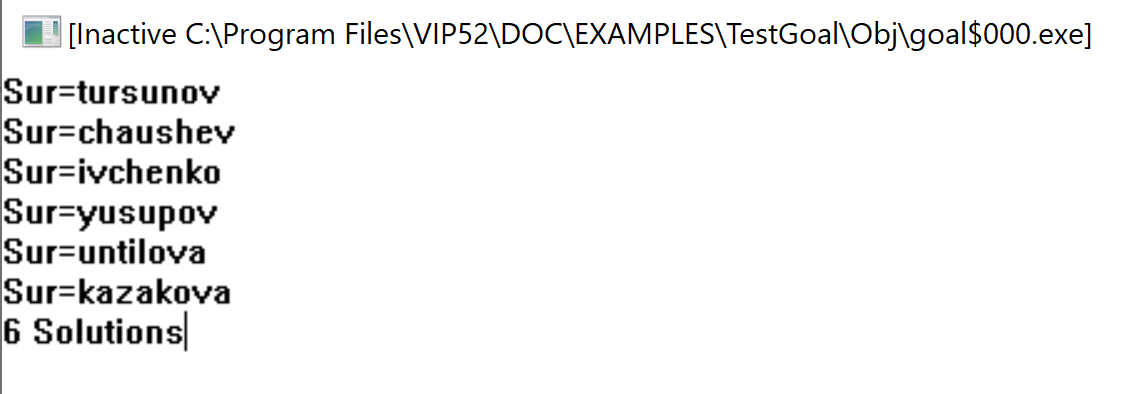
\includegraphics[scale=1]{2.1}
	\centering\caption{Вопрос: group (Sur, iu766).}
\end{figure}

\begin{figure}[h!]
	\centering 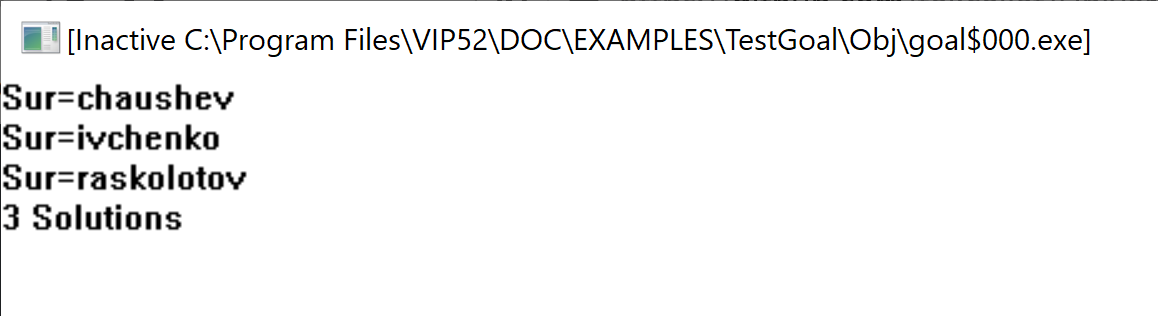
\includegraphics[scale=1]{2.2}
	\centering\caption{Вопрос: district (Sur, izmaylovo).}
\end{figure}

\begin{figure}[h!]
	\centering 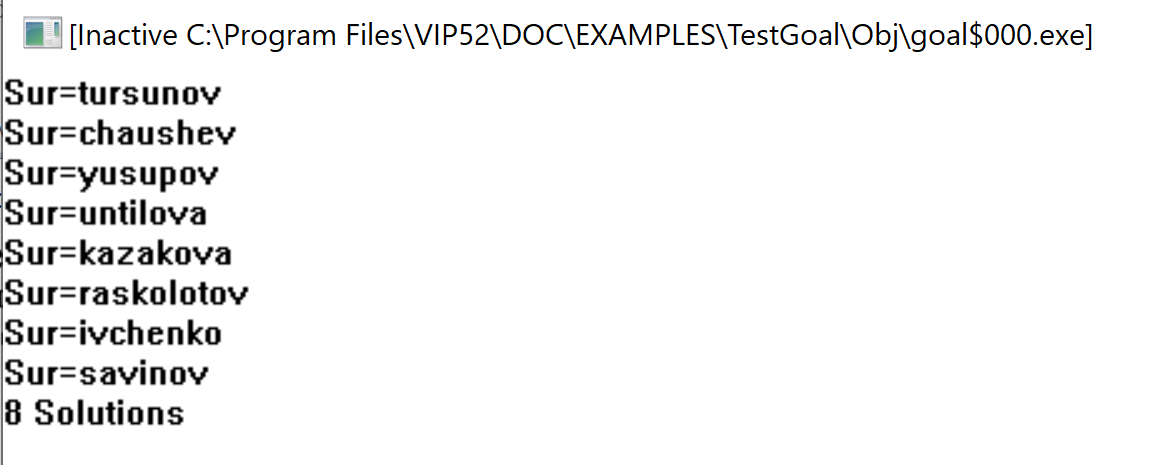
\includegraphics[scale=1]{2.3}
	\centering\caption{Вопрос: grantL(Sur).}
\end{figure}

\section*{Задание 3}
\addcontentsline{toc}{section}{Задание 3}
Составить программу, т.е. модель предметной области – базу знаний, объединив в ней информацию – знания:
\begin{itemize}
	\item «Телефонный справочник»: Фамилия, №тел, Адрес – структура (Город, Улица, №дома, №кв);
	\item «Автомобили»: $Фамилия_{владельца}$, Марка, Цвет, Стоимость, и др.;
	\item «Вкладчики банков»: Фамилия, Банк, счет, сумма, др.
\end{itemize}	
Владелец может иметь несколько телефонов, автомобилей, вкладов (Факты).
Используя правила, обеспечить возможность поиска:
\begin{enumerate}
	\item \begin{itemize}
		\item По № телефона найти: Фамилию, Марку автомобиля, Стоимость автомобиля (может быть несколько);
		\item Используя сформированное в пункте а) правило, по № телефона найти: только Марку автомобиля (автомобилей может быть несколько).
	\end{itemize}
	\item Используя простой, не составной вопрос: по Фамилии (уникальна в городе, но в разных городах есть однофамильцы) и Городу проживания найти:  Улицу проживания, Банки, в которых есть вклады и №телефона.
\end{enumerate}
Для задания1 и задания 2:
\\ \hspace*{5mm} Для одного из вариантов ответов, и для а) и для в), описать словесно порядок поиска ответа на вопрос, указав, как выбираются знания, и, при этом, для каждого этапа унификации, выписать подстановку – наибольший общий унификатор, и соответствующие примеры термов.


\begin{lstlisting}
domains
	surname, number, city, street, brand, model, color, bank, account = symbol.
	price, money = integer.
	address_t = address(city, street, integer, integer).

predicates
	person(surname, number, address_t).
	car(surname, brand, model, color, price).
	deposit(surname, address_t, bank, account, money).
	all_by_phone(number, surname, brand, price).
	brand_by_phone(number, brand).
	by_surname_city(surname, city, street, bank, number).

clauses
	person("Ivanov", "000-000", address("Example", "street", 0, 0)).
	person("Ivanov", "111-111", address("City-17", "Gordon street", 0, 0)).
	person("Petrov", "001-917", address("St. Petersburg", "Lenina", 24, 42)).
	person("Sidorov", "555-555", address("Los Angeles", "Apple street", 0, 1)).
	person("A", "123-456", address("B", "C avnenue", 13, 14)).
	person("Another", "123-321", address("One", "Good street", 3, 12)).
	person("One", "999-666", address("More", "Pioneer street", 3, 4)).
	person("Not", "987-654", address("Enough", "Bad Fantasy avenue", 9, 9)).

	car("Ivanov", "Bugatti", "La Voiture Noire", "Black", 1178000).
	car("Ivanov", "Aston Martin", "Valkyrie", "Grey", 230000).
	car("Petrov", "Lada", "Kalina", "White", 200).
	car("Sidorov", "Ford", "Focus", "Red", 400).

	deposit("Ivanov", address("Example", "street", 0, 0), 
		"Sberbank", "0-0-0-0", 999999999).
	deposit("Ivanov", address("Example", "street", 0, 0), 
		"VTB", "0-0-0-1", 1).
	deposit("Ivanov", address("City-17", "Gordon street", 0, 0), 
		"Tinkoff", "0-1-0-1", 987654).
	deposit("Petrov", address("St. Petersburg", "Lenina", 24, 42), 
		"Alfa", "1-2-3-4", 999999999).
	deposit("Sidorov", address("Los Angeles", "Apple street", 0, 1), 
		"Mavrodi", "6-9-6-9", 1).


	by_surname_city(Surname, City, Street, Bank, Number) :- 
		person(Surname, Number, address(City, Street, _, _)), 
		deposit(Surname, address(City, Street, _, _), Bank, _, _).
	person("Another", "123-321", address("One", "Good street", 3, 12)).
	person("One", "999-666", address("More", "Pioneer street", 3, 4)).
	person("Not", "987-654", address("Enough", "Bad Fantasy avenue", 9, 9)).

	car("Ivanov", "Bugatti", "La Voiture Noire", "Black", 1178000).
	car("Ivanov", "Aston Martin", "Valkyrie", "Grey", 230000).
	car("Petrov", "Lada", "Kalina", "White", 200).
	car("Sidorov", "Ford", "Focus", "Red", 400).

	deposit("Ivanov", address("Example", "street", 0, 0), 
		"Sberbank", "0-0-0-0", 999999999).
	deposit("Ivanov", address("Example", "street", 0, 0), 
		"VTB", "0-0-0-1", 1).
	deposit("Ivanov", address("City-17", "Gordon street", 0, 0), 
		"Tinkoff", "0-1-0-1", 987654).
	deposit("Petrov", address("St. Petersburg", "Lenina", 24, 42), 
		"Alfa", "1-2-3-4", 999999999).
	deposit("Sidorov", address("Los Angeles", "Apple street", 0, 1), 
		"Mavrodi", "6-9-6-9", 1).
	deposit("Another", address("One", "Good street", 3, 12), 
		"Bankname", "10-20-30-40", 40302010).

	all_by_phone(Number, Surname, Brand, Price) :- person(Surname, Number, _), 
		car(Surname, Brand, _, _, Price).
	brand_by_phone(Number, Brand) :- all_by_phone(Number, _, Brand, _).
	by_surname_city(Surname, City, Street, Bank, Number) :- 
		person(Surname, Number, address(City, Street, _, _)), 
		deposit(Surname, address(City, Street, _, _), Bank, _, _).

goal
	%all_by_phone("000-000", Surname, Brand, Price).    
	%brand_by_phone("000-000", Brand).
	%by_surname_city("Ivanov", "Example", Street, Bank, Number).

\end{lstlisting}

\subsubsection*{Примеры работы:}
Surname=Ivanov, Brand=Bugatti, Price=11780000
\\Surname=Ivanov, Brand=Aston Martin, Price=2300000
\\2 Solutions

Ответ на вопрос all by phone("000-000", Surname, Brand, Price).
\\Brand=Bugatti
\\Brand=Aston Martin
\\2 Solutions

Ответ на вопрос brand by phone("000-000", Brand).
\\Street=street, Bank=Sberbank, Number=000-000
\\Street=street, Bank=VTB, Number=000-000
\\2 Solutions

Ответ на вопрос by surname city("Ivanov", "Example", Street, Bank, Number).

\clearpage
\newpage
Описание порядка поиска ответа.
\\ 1) all by phone("000-000", Surname, Brand, Price).

\begin{figure}[h!]
	\centering 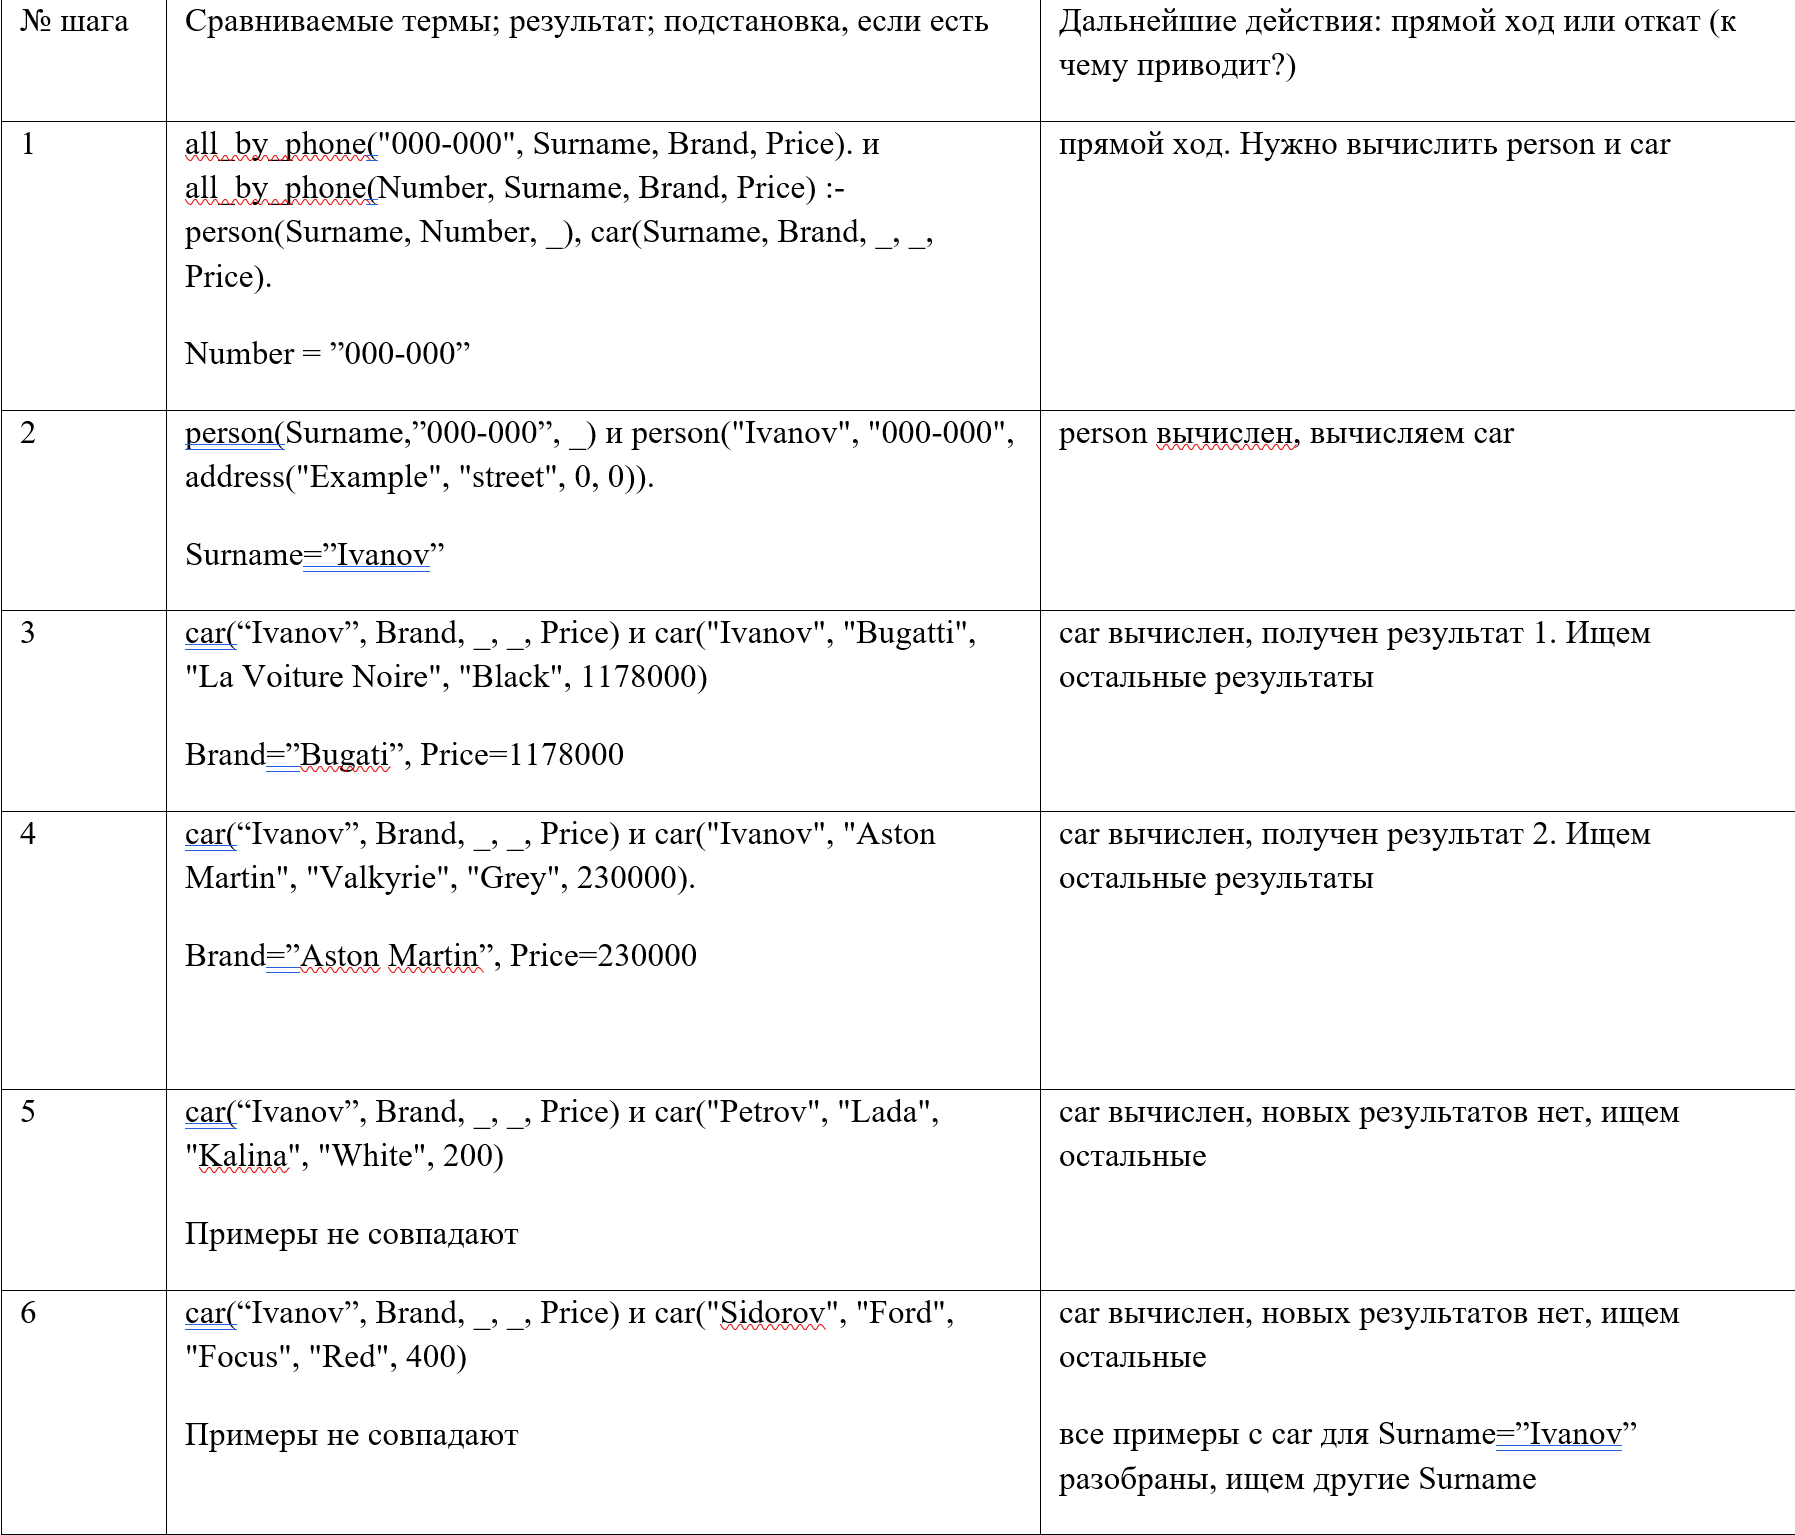
\includegraphics[scale=0.8]{3.1}
\end{figure}
\begin{figure}[h!]
	\centering 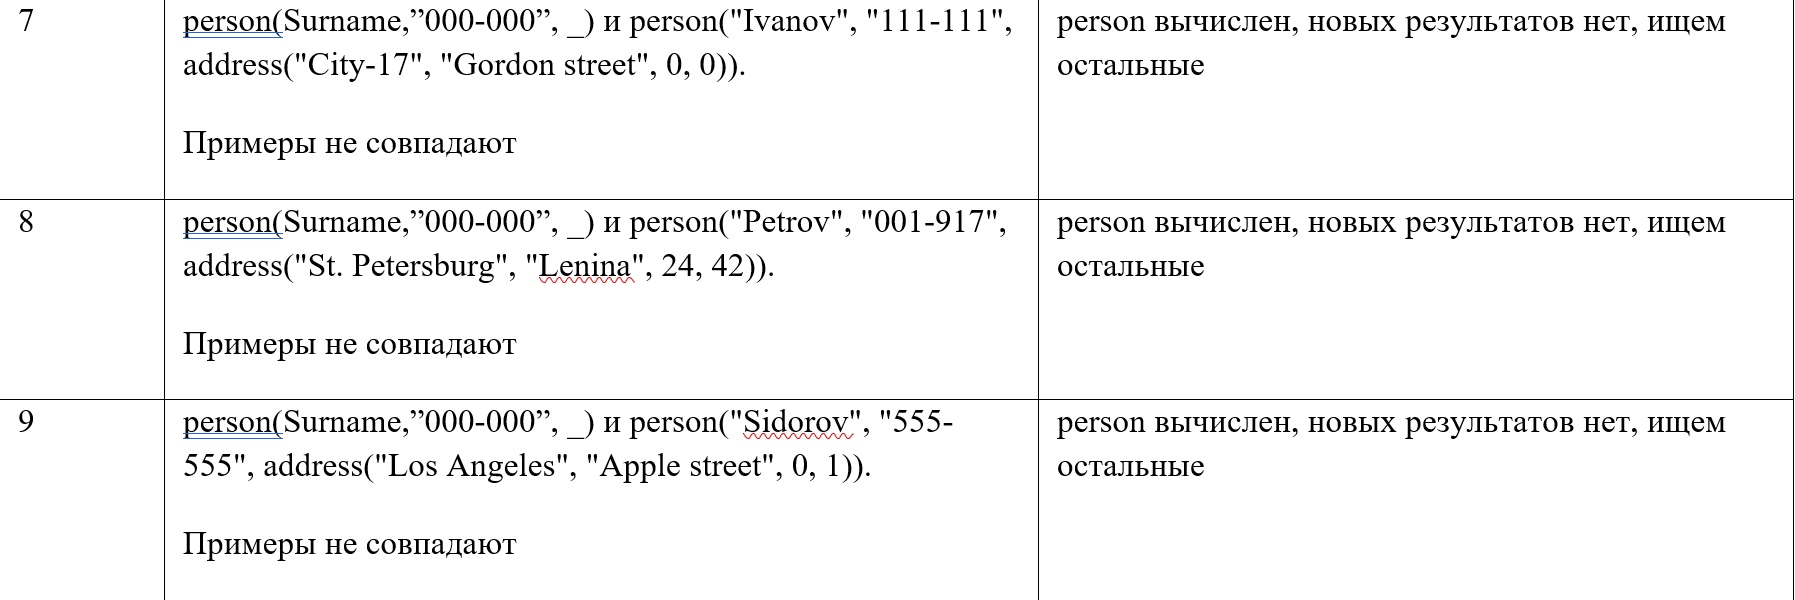
\includegraphics[scale=0.8]{3.2}
\end{figure}
\clearpage
\newpage
\begin{figure}[h!]
	\centering 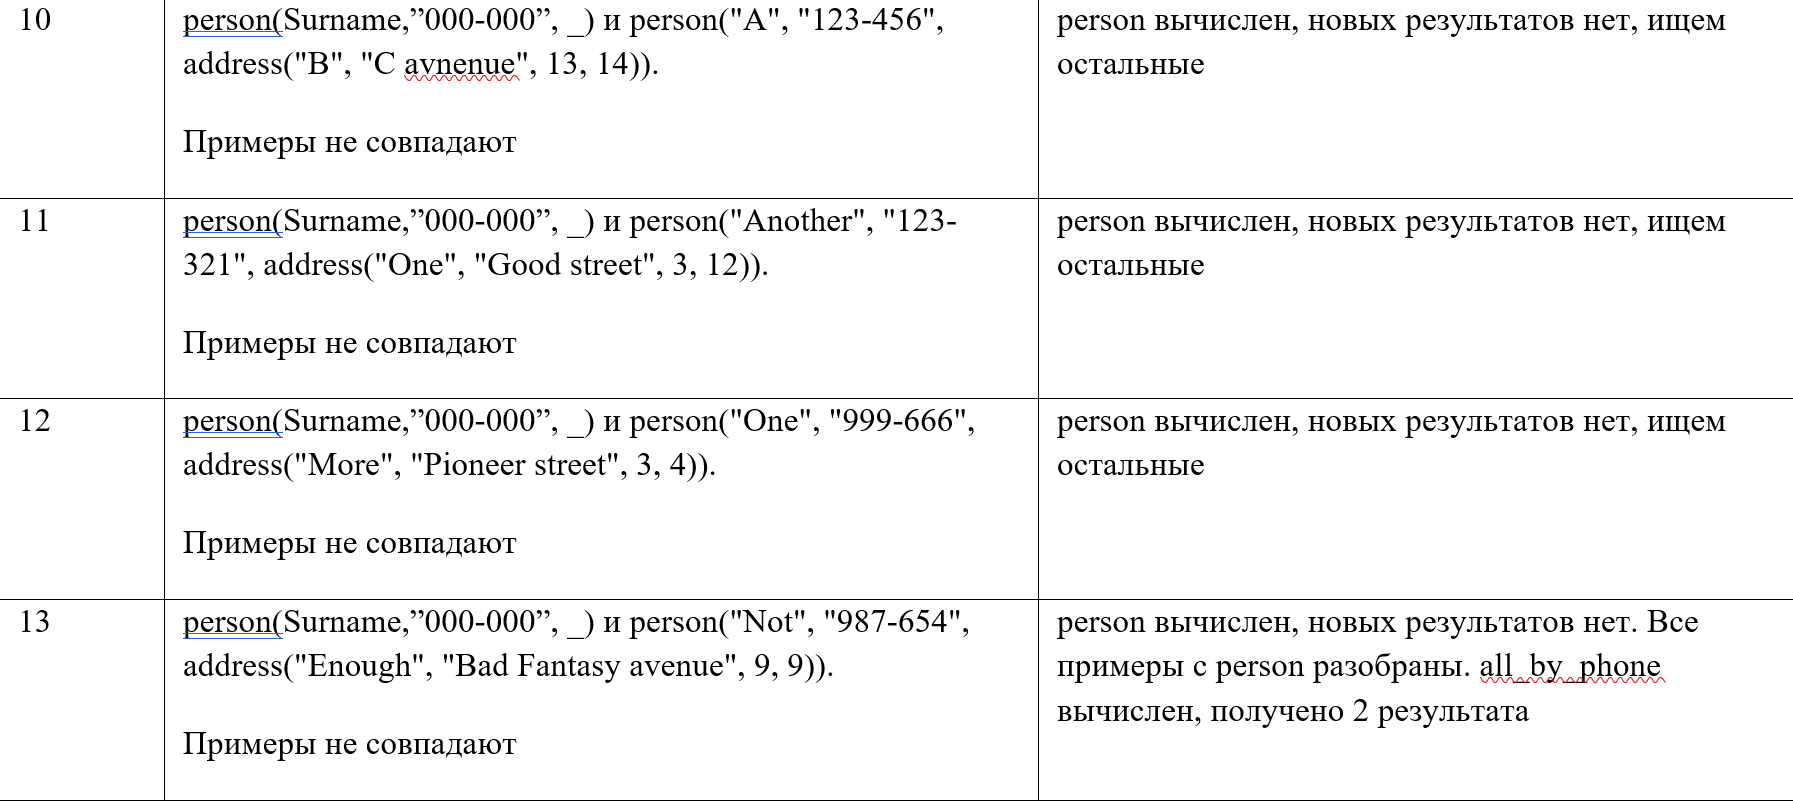
\includegraphics[scale=0.8]{3.3}
\end{figure}

2) brand by phone("000-000", Brand).

\begin{figure}[h!]
	\centering 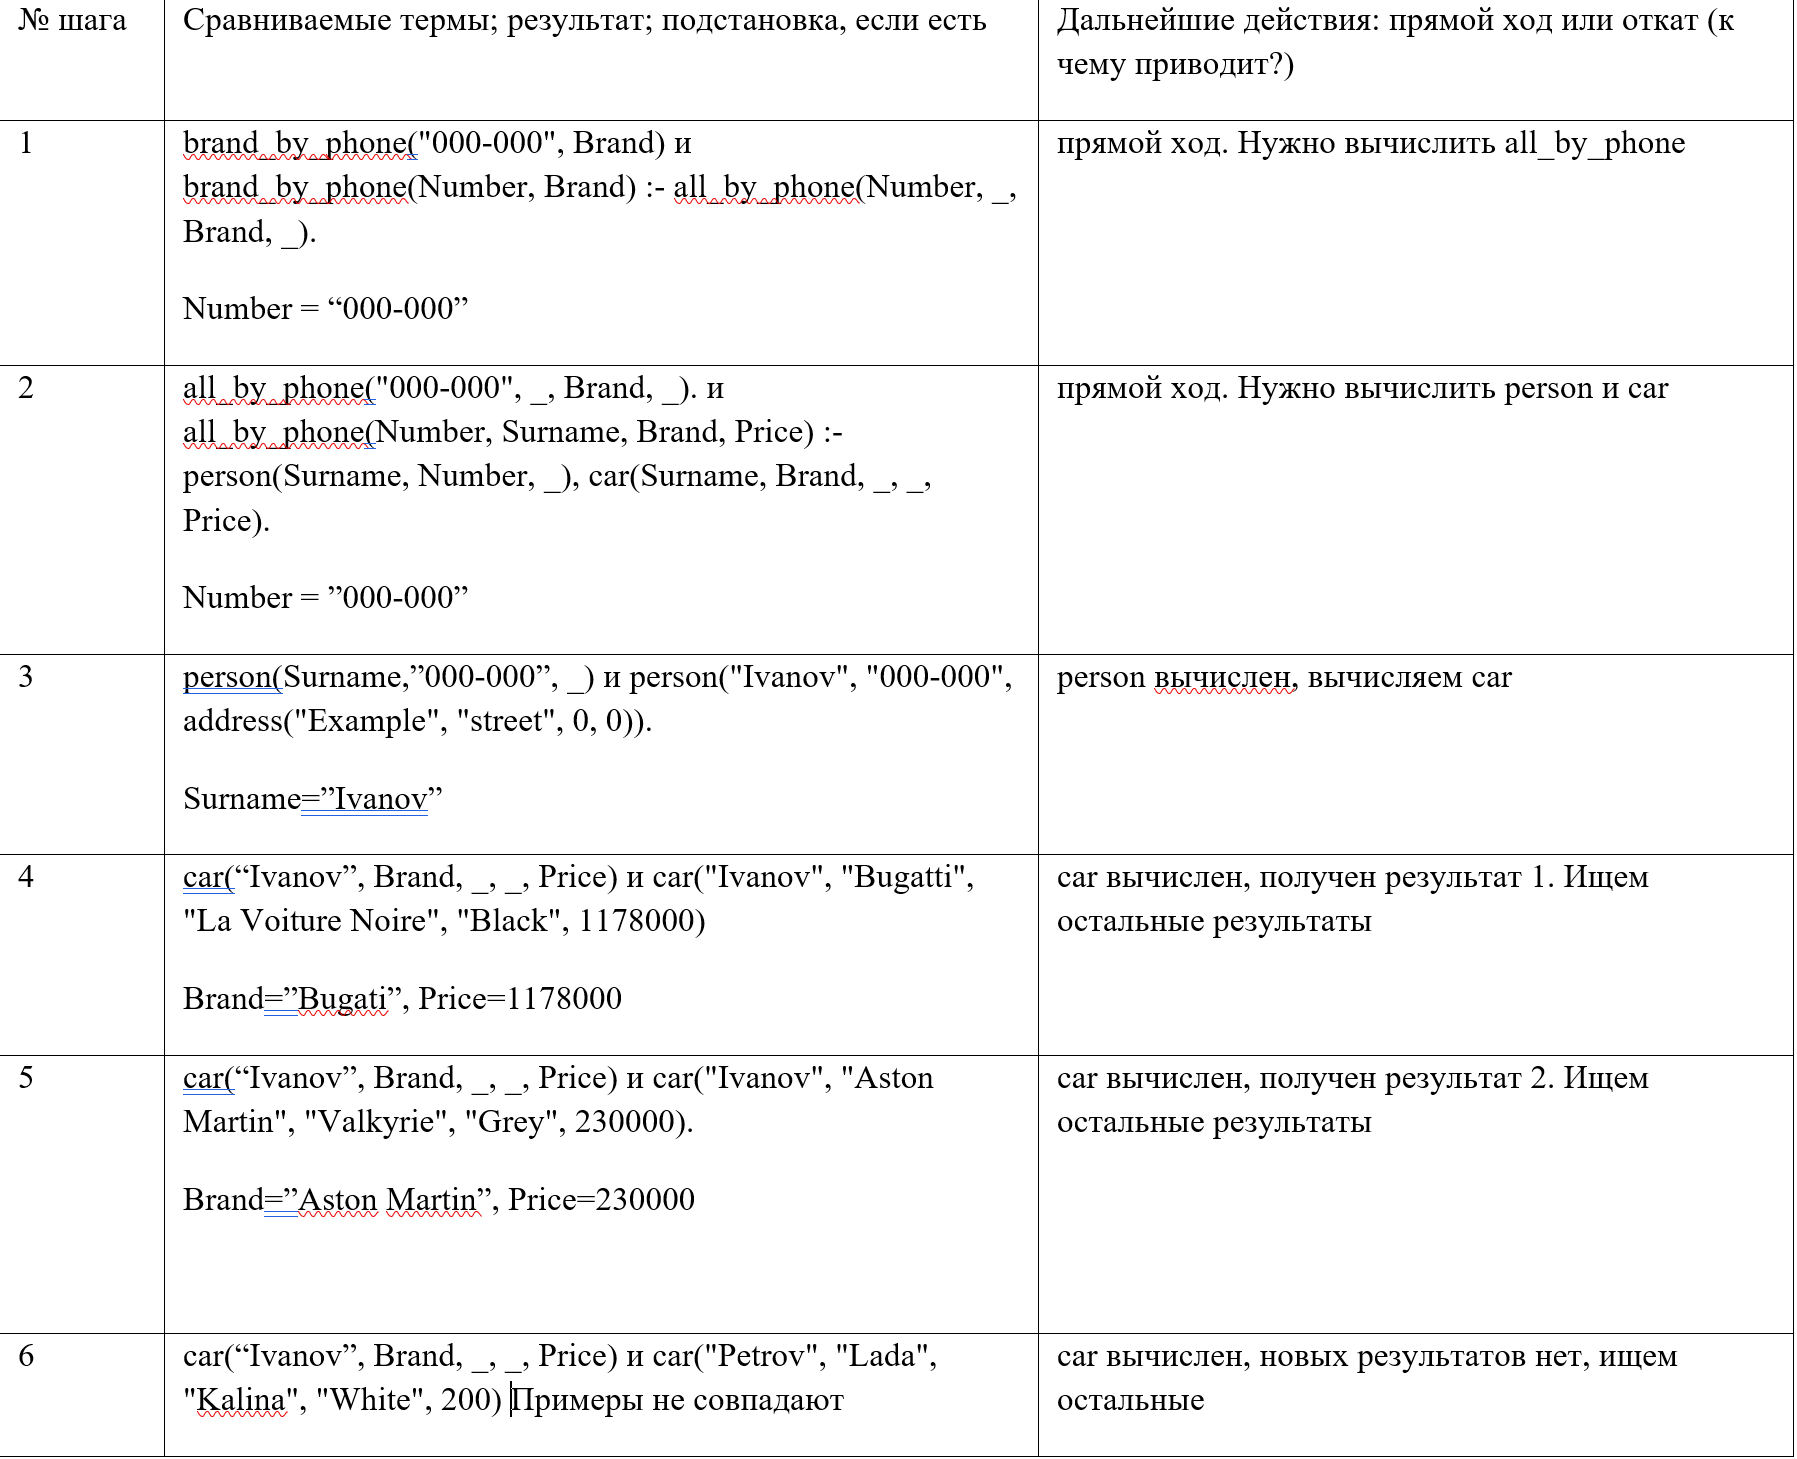
\includegraphics[scale=0.8]{3.4}
\end{figure}
\clearpage
\newpage
\begin{figure}[h!]
	\centering 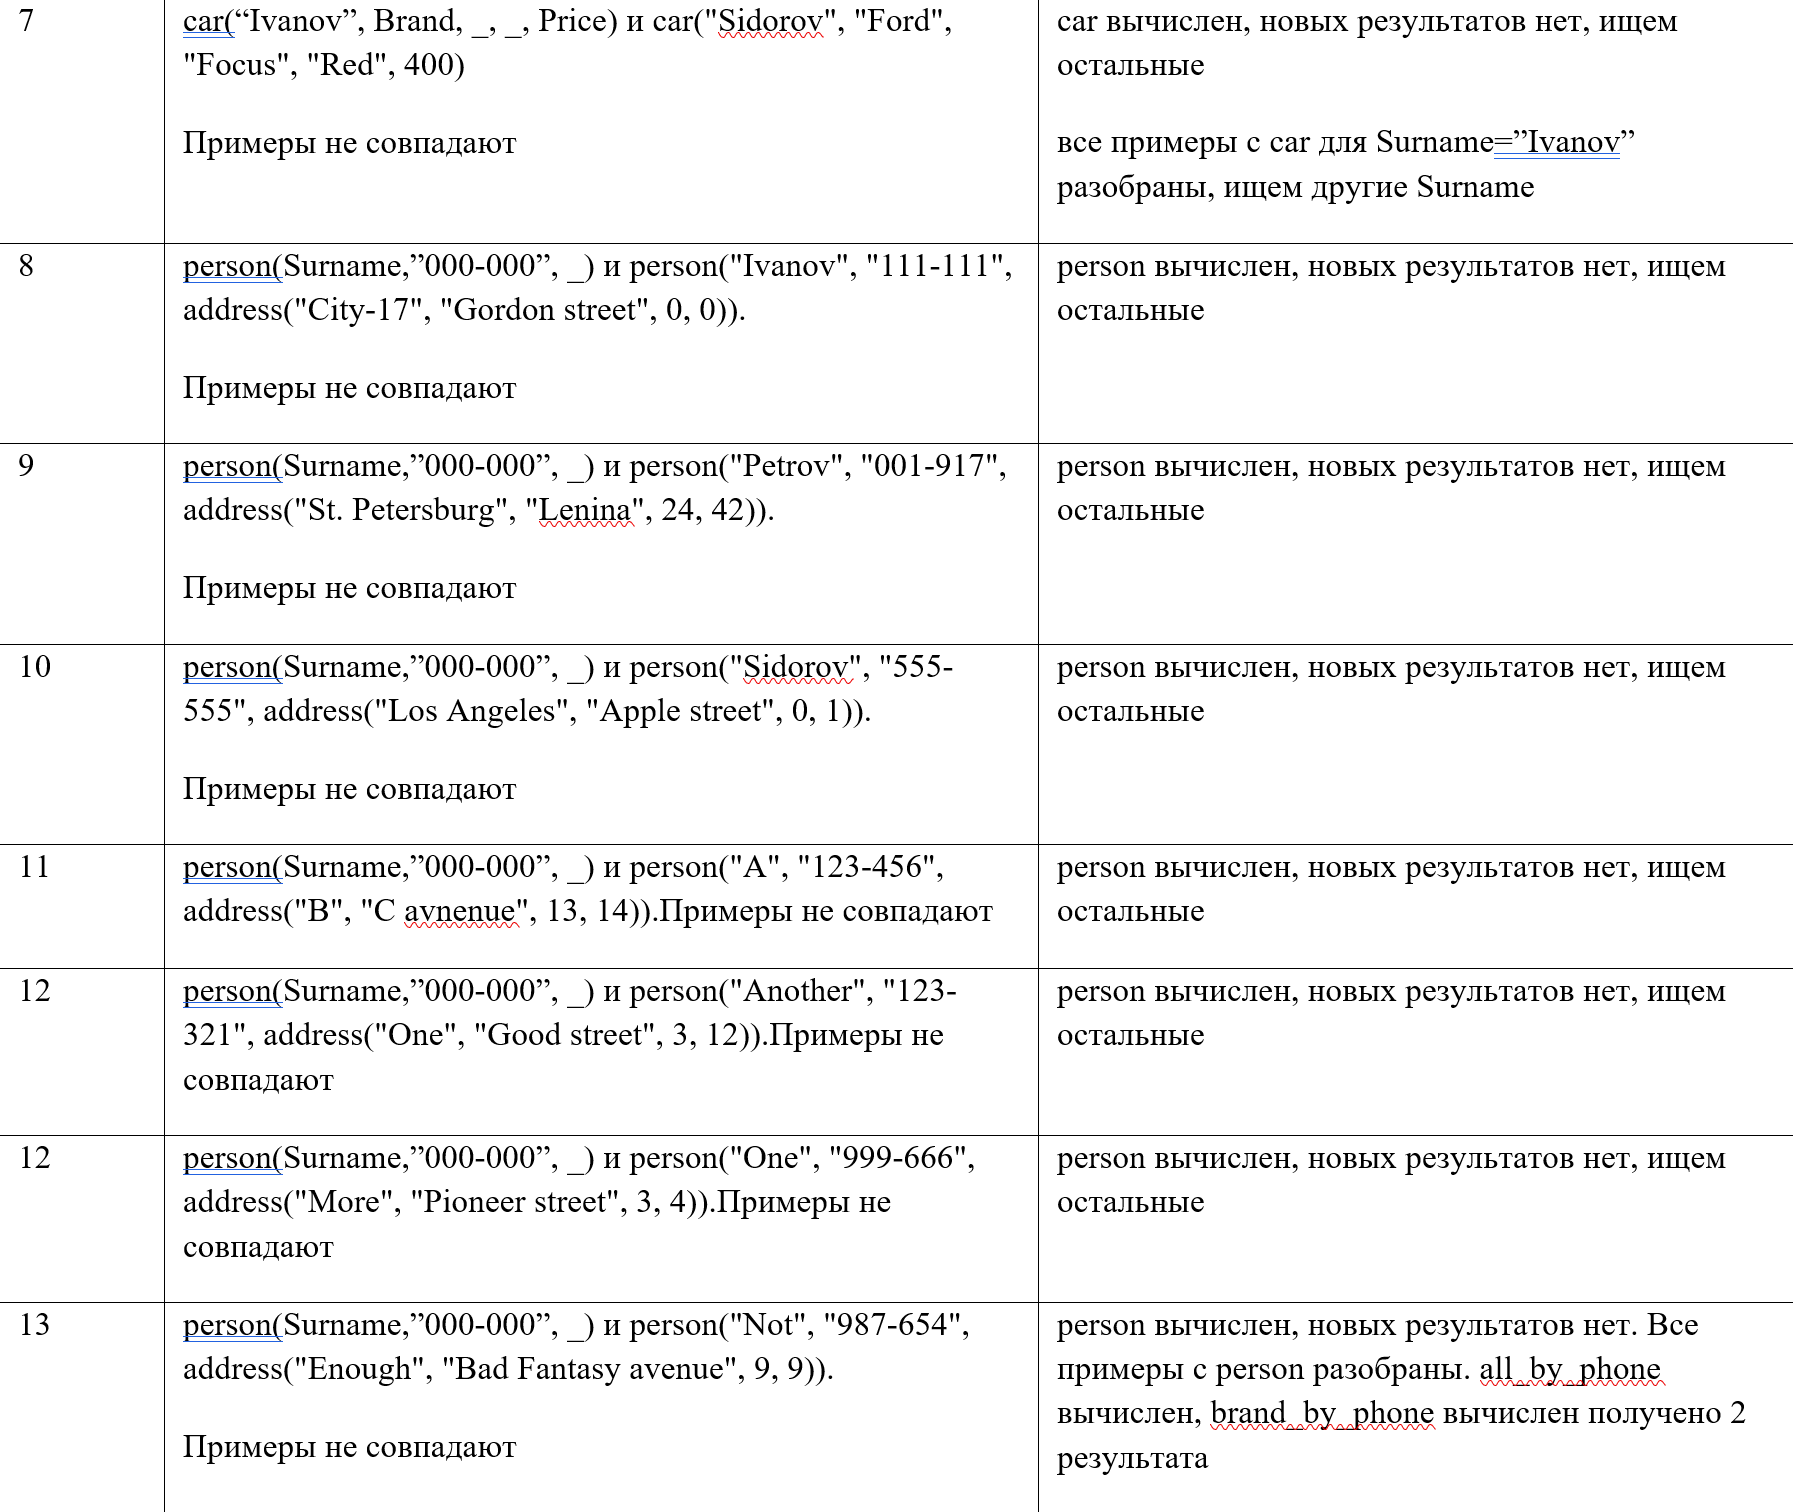
\includegraphics[scale=0.8]{3.5}
\end{figure}
3) by surname city("Ivanov", "Example", Street, Bank, Number).
\begin{figure}[h!]
	\centering 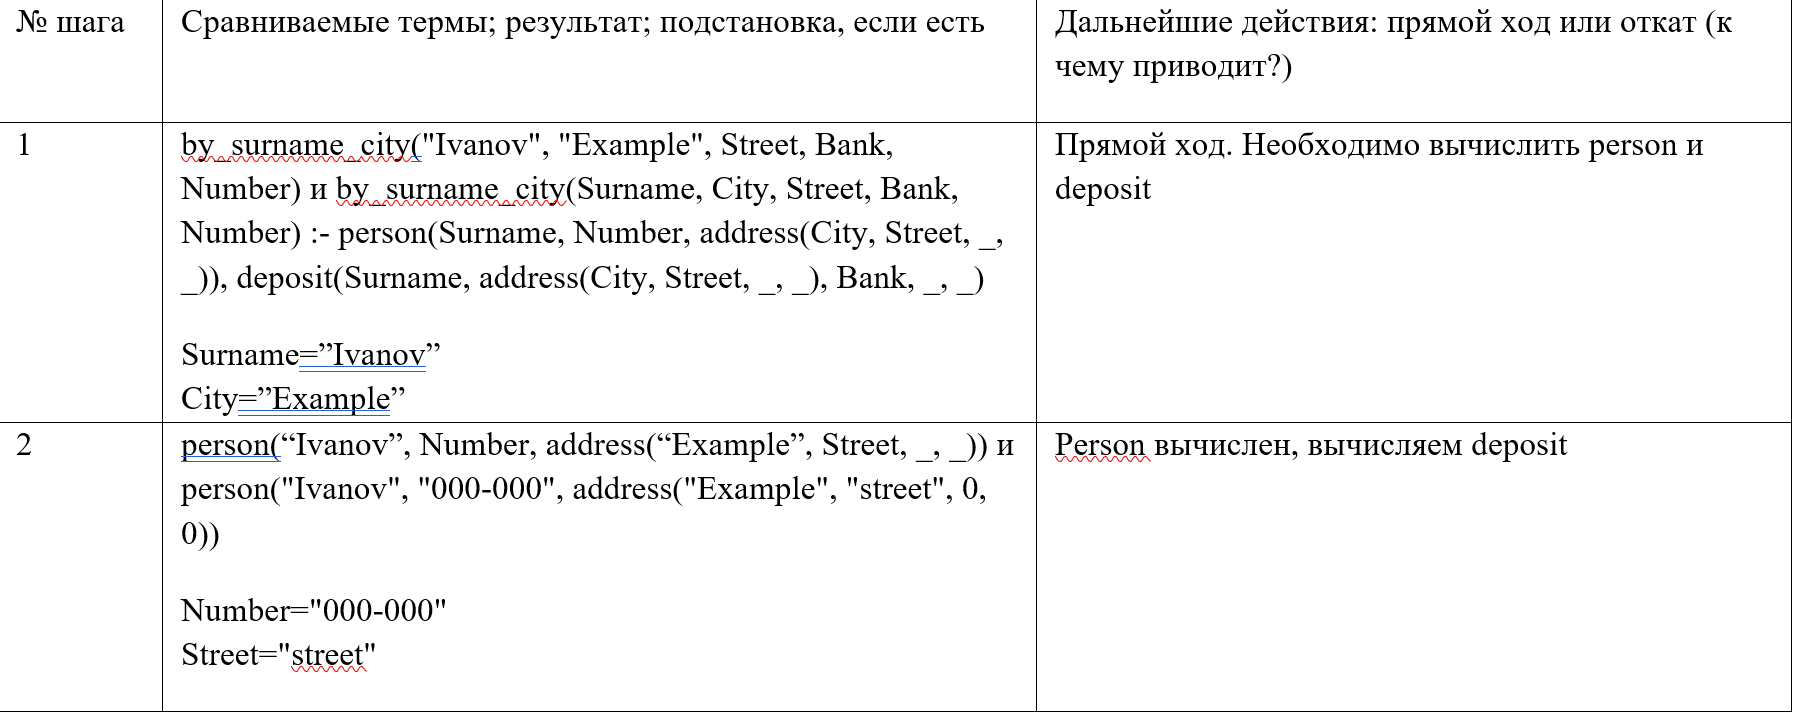
\includegraphics[scale=0.8]{3.6}
\end{figure}
\clearpage
\newpage
\begin{figure}[h!]
	\centering 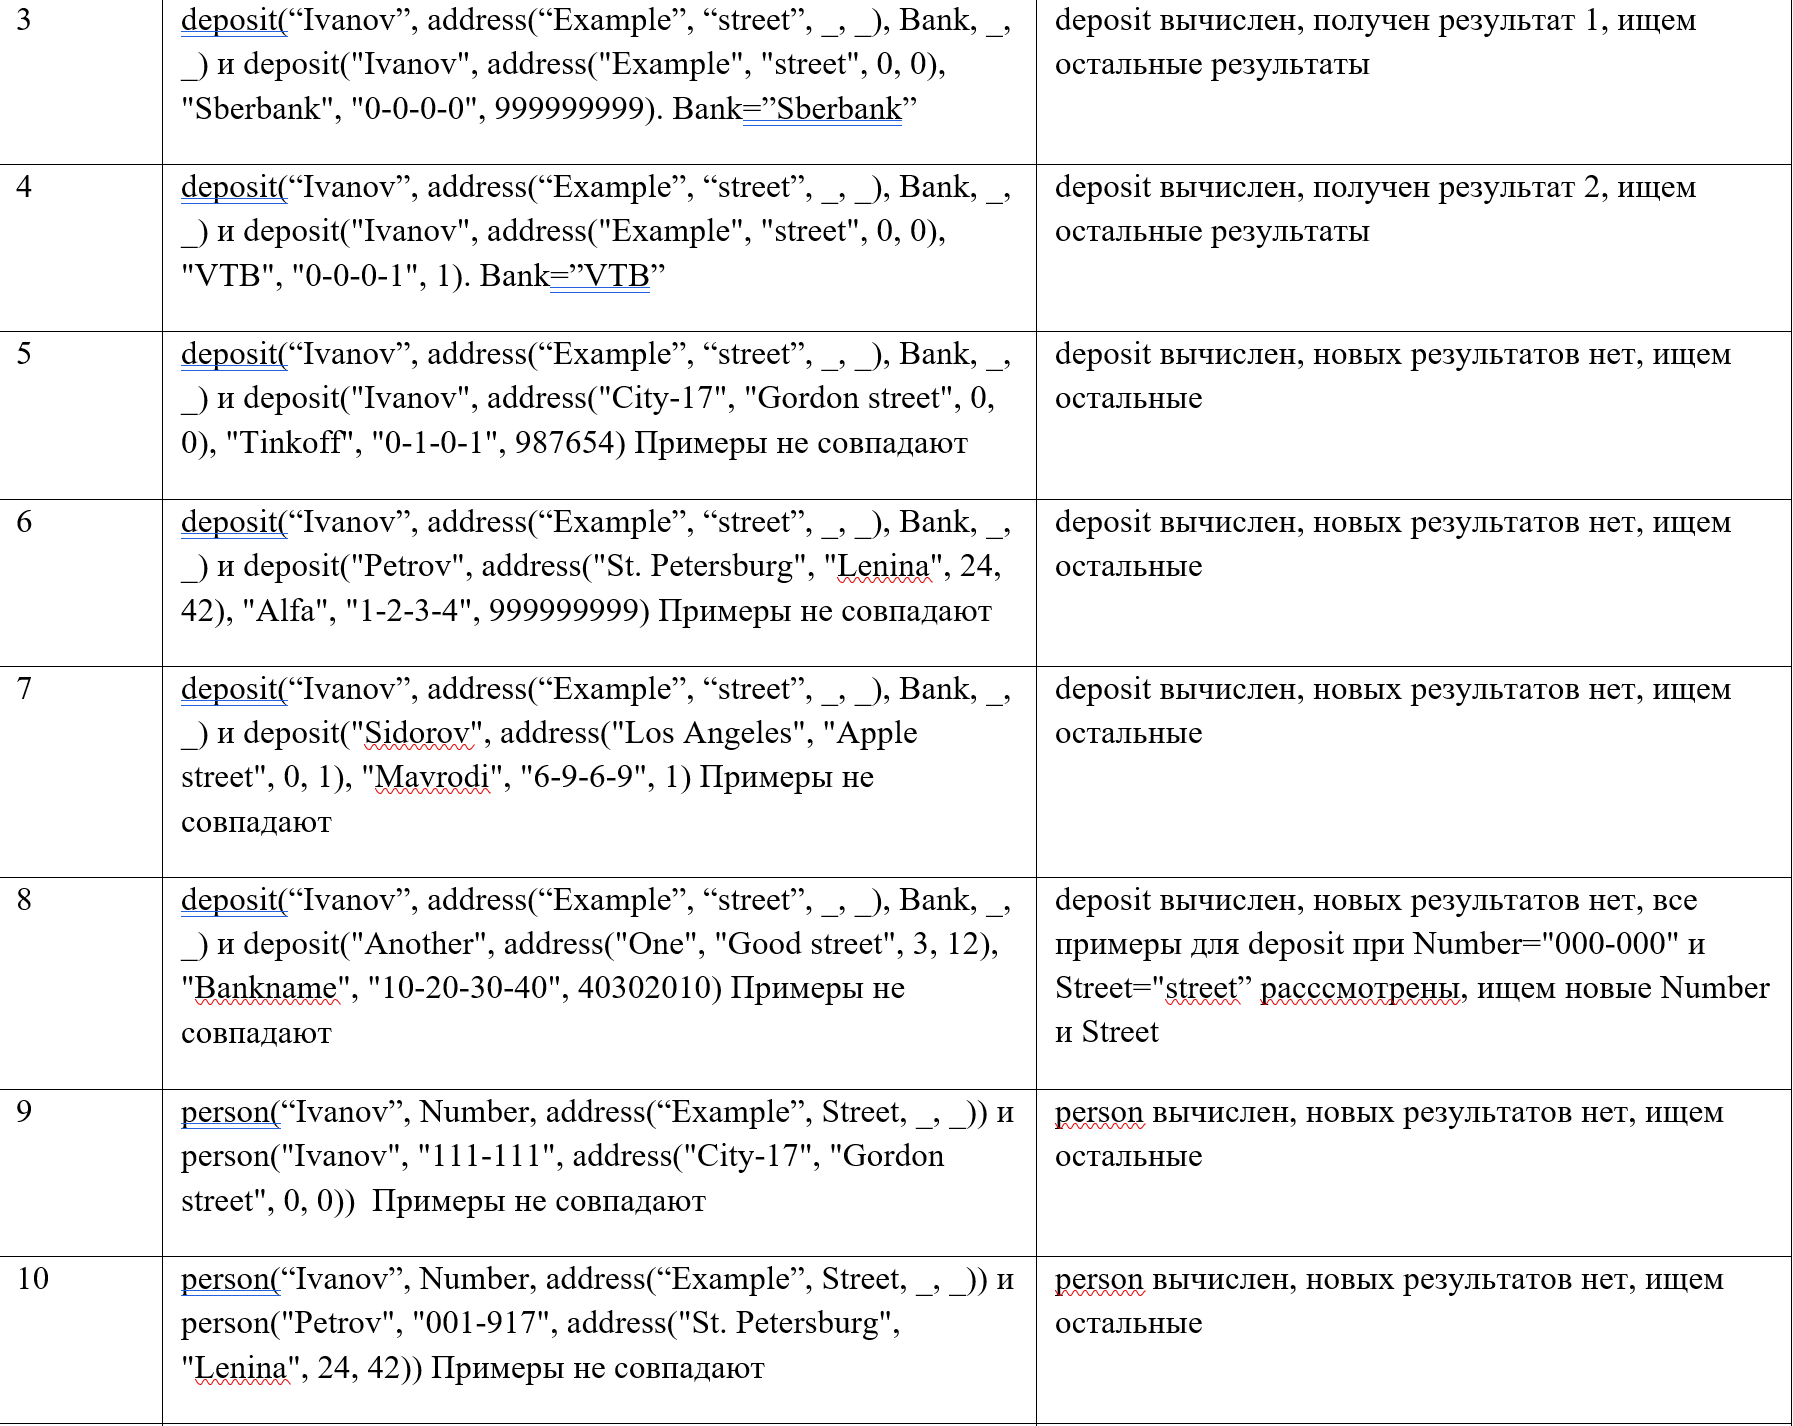
\includegraphics[scale=0.8]{3.7}
\end{figure}
\begin{figure}[h!]
	\centering 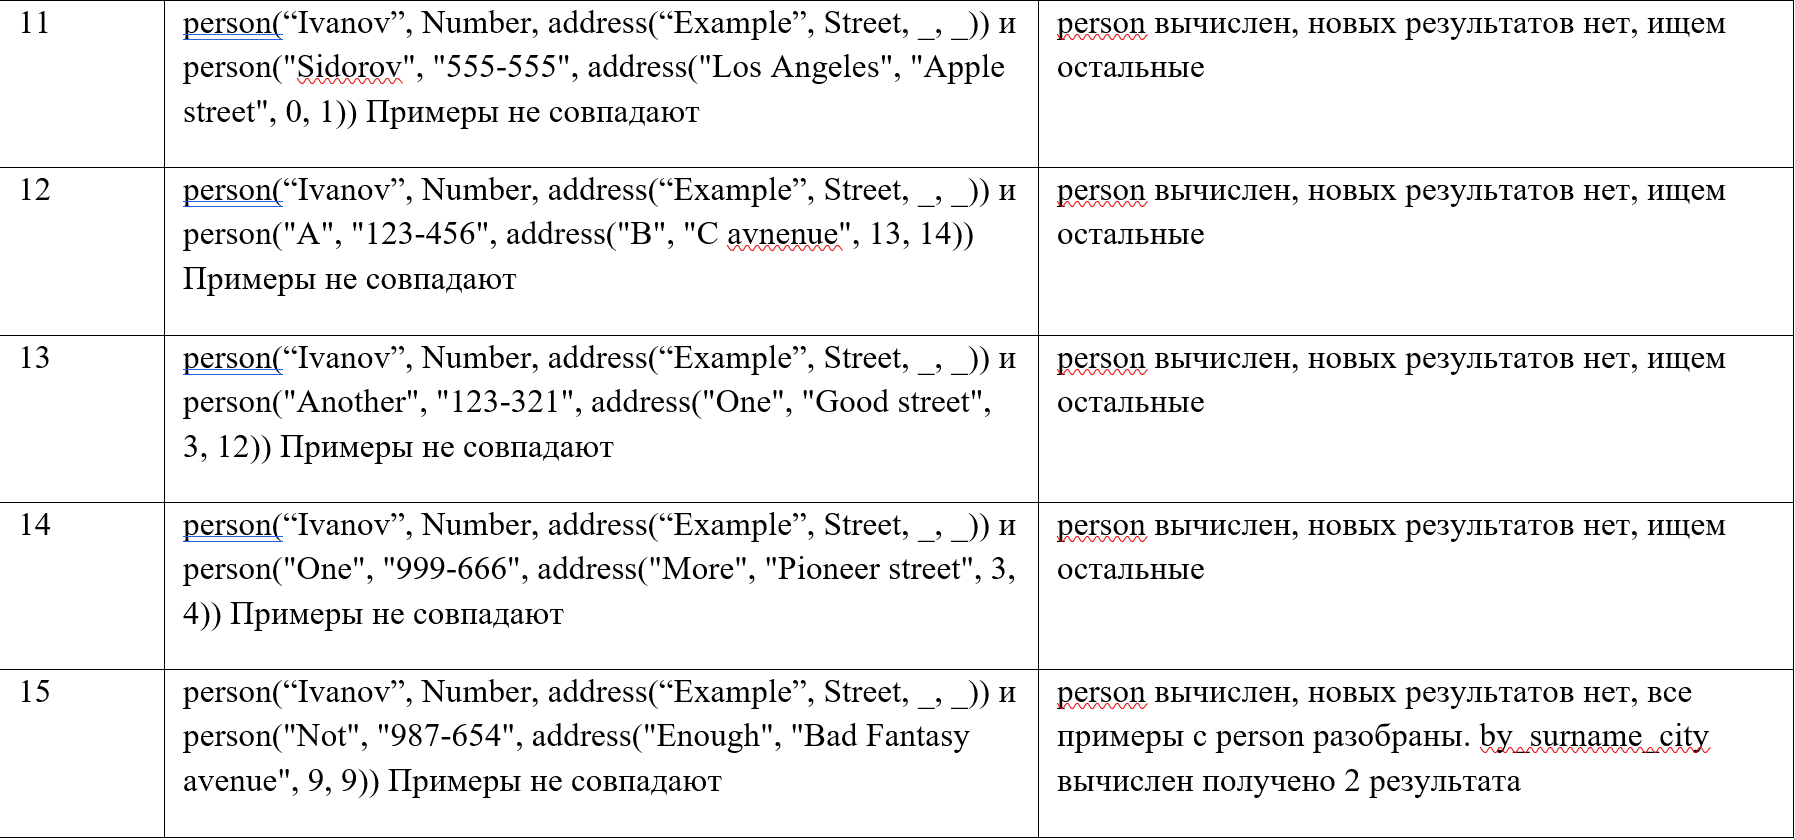
\includegraphics[scale=0.8]{3.8}
\end{figure}

\section*{Ответы на вопросы:}
\addcontentsline{toc}{section}{Ответы на вопросы}
\hspace*{-7mm} \textbf{1) Что такое терм?}
\\ Терм – основной элемент языка Prolog. Может быть константой (число, символьный атом, строка), преременной (именованной или анонимной) или составным термом (функтуатор(терм1, терм2, ...)).


\hspace*{-13mm} \textbf{2) Что такое предикат в матлогике (математике)?}
\\ Предикат (n -местный, или n-арный) — это функция с множеством значений {0, 1} (или {ложь, истина}), определённая на множестве M = M1×M2×…×Mn. Таким образом, каждый набор элементов множества M характеризуется либо как «истинный», либо как «ложный».


\hspace*{-13mm} \textbf{3) Что описывает предикат в Prolog?}
\\ В Prolog предикат описывает общий вид фактов и правил.

\hspace*{-13mm} \textbf{4) Назовите виды предложений в программе и приведите примеры таких предложений из Вашей программы. Какие предложения являются основными, а какие – не основными?  Каковы: синтаксис и семантика (формальный смысл) этих предложений (основных и неосновных)?}
\\ Предложение может быть фактом или правилом. Предложения бывают основные (не содержащие переменные) и неосновные (содержащие).
\\ Пример:
	\\1) person("Ivanov", "000-000", address("Example", "street", 0, 0)). - основное
	all\_by\_phone(Number, Surname, Brand, Price) :- person(Surname, Number, \_), car(Surname, Brand, \_, \_, Price). – неосновное (правило)
	\\ all\_by\_phone("000-000", Surname, Brand, Price). – неосновное (запрос)
	синтаксис основных: имя\_предиката(значение1, значение2, ...).
	синтаксис неосновных: имя\_предиката(значение/имя\_переменной, ...).
	
\hspace*{-13mm} \textbf{5) Каковы назначение, виды и особенности использования переменных в программе на Prolog? Какое предложение БЗ сформулировано в более общей – абстрактной форме: содержащее или не содержащее переменных?}
\\ Переменная обозначает даныне, одинаковые внутри предложения. Переменные должны начинаться с большой буквы или символа подчеркивания и состоять только из симвалов латинского алфавита и символов подчеркивания. Переменные бывают именованные и аномные (их имя – один символ «\_»). Предложение, сформулированное с помощью переменных, является более абстрактным, так как не требует заранее зафиксированного значения, а лишь описывает, какие значения должны совпадать. Соответственно, по запросам с разными значениями одни и те же предложения могут давать разные ответы, если были описаны с переменными.

\hspace*{-13mm} \textbf{6) Что такое подстановка?}
\\ Подстановка – набор термов t1, t2, ..., tN, подставляемых в терм A(X1, X2, ..., XN). Применение подстановки заключается в замене каждого вхождения переменной xi  на соответствующий терм. Пусть $\delta$ =  { x 1 = t 1, x 2= t 2, … , x n = tn } – подстановка. Обозначение ее результата: A$\delta$.

\hspace*{-13mm} \textbf{7) Что такое пример терма? Как и когда строится? Как Вы думаете, система строит и хранит примеры?}
\\ Терм В называется примером терма А, если существует такая подстановка $\delta$, что В=А$\delta$.
Вероятно, система строит примеры при вычислении ответа на вопрос, и может их хранить, если в данном правиле часто идет обращение  к данному примеру.


\end{document}